\documentclass[uplatex,a4j,11pt,dvipdfmx]{jsarticle}
\usepackage{listings,jvlisting}
\bibliographystyle{junsrt}

\usepackage{url}

\usepackage{graphicx}
\usepackage{gnuplot-lua-tikz}
\usepackage{pgfplots}
\usepackage{tikz}
\usepackage{amsmath,amsfonts,amssymb}
\usepackage{bm}
\usepackage{siunitx}

\makeatletter
\def\fgcaption{\def\@captype{figure}\caption}
\makeatother
\newcommand{\setsections}[3]{
\setcounter{section}{#1}
\setcounter{subsection}{#2}
\setcounter{subsubsection}{#3}
}
\newcommand{\mfig}[3][width=15cm]{
\begin{center}
\includegraphics[#1]{#2}
\fgcaption{#3 \label{fig:#2}}
\end{center}
}
\newcommand{\gnu}[2]{
\begin{figure}[hptb]
\begin{center}
\input{#2}
\caption{#1}
\label{fig:#2}
\end{center}
\end{figure}
}
\newcommand{\gaa}{\gamma_{AA}}
\newcommand{\gbb}{\gamma_{BB}}
\newcommand{\gab}{\gamma_{AB}}

\begin{document}
\title{磁性物理学 レポート No.5}
\author{82311971 佐々木良輔}
\date{}
\maketitle
${\bm M}=(m_xe^{i\omega t},m_ye^{i\omega t},M_s)$, ${\bm H}=(0,he^{i\omega t}, H_0)$としたとき,
LLG方程式の$x$成分, $y$成分はそれぞれ
\begin{align}
  i\omega m_x+(\gamma H_0+i\omega\alpha)m_y&=\gamma M_s h\\
  (\gamma H_0+i\omega \alpha)m_x-i\omega m_y&=0
\end{align}
であった. (1)式から$m_y$を削除すると
\begin{align}
  {
    \everymath{\displaystyle}
    \begin{array}{cc}
      &\gamma M_sh=i\omega m_x+(\gamma H_0+i\omega\alpha)\frac{\gamma H_0+i\omega\alpha}{i\omega}m_x\\
      \iff&m_x=\frac{i\omega\gamma M_s}{-\omega^2+(\gamma H_0+i\omega\alpha)^2}h\\
    \end{array}
  }
\end{align}
ここで$\gamma H_0=\omega_0$を用いると
\begin{align}
  \begin{split}
    m_x&=\frac{i\omega\gamma M_s}{-\omega^2+(\omega_0+i\omega\alpha)^2}h\\
    &=\frac{i\omega\gamma M_s}{\omega_0^2-(1+\alpha^2)\omega^2+2i\omega\omega_0\alpha}h\\
    &=\frac{i\omega\gamma M_s\left(\omega_0^2-(1+\alpha^2)\omega^2-2i\omega\omega_0\alpha\right)}
    {\left(\omega_0^2-(1+\alpha^2)\omega^2\right)^2+4\omega^2\omega_0^2\alpha^2}h\\
    &=\chi_{xy}h
  \end{split}
\end{align}
したがって$\chi_{xy}$の実部,虚部はそれぞれ
\begin{align}
  \Re(\chi_{xy})=\frac{2\omega^2\omega_0\alpha\gamma M_s}
  {\left(\omega_0^2-(1+\alpha^2)\omega^2\right)^2+4\omega^2\omega_0^2\alpha^2}
\end{align}
\begin{align}
  \Im(\chi_{xy})=\frac{\omega\gamma M_s(\omega_0^2-(1+\alpha^2)\omega^2)}
  {\left(\omega_0^2-(1+\alpha^2)\omega^2\right)^2+4\omega^2\omega_0^2\alpha^2}
\end{align}
となる.図1にこれらのグラフを示す.
ただし$\omega_0=3$, $\alpha=0.02$, $M_s=0.5$, $g=2$とした.プロットにはDesmosを用いた.

次に$m_y$は(2)式と(4)式から
\begin{align}
  \begin{split}
    m_y&=\frac{\omega_0+i\omega\alpha}{i\omega}m_x\\
    &=\frac{\omega_0+i\omega\alpha}{i\omega}
    \frac{i\omega\gamma M_s\left(\omega_0^2-(1+\alpha^2)\omega^2-2i\omega\omega_0\alpha\right)}
    {\left(\omega_0^2-(1+\alpha^2)\omega^2\right)^2+4\omega^2\omega_0^2\alpha^2}h\\
    &=\gamma M_s\frac{
      \omega_0\left(\omega_0^2-(1+\alpha^2)\omega^2\right)-2i\omega\omega_0^2\alpha+
      i\omega\alpha\left(\omega_0^2-(1+\alpha^2)\omega^2\right)+2\omega_0\omega^2\alpha^2
    }{\left(\omega_0^2-(1+\alpha^2)\omega^2\right)^2+4\omega^2\omega_0^2\alpha^2}h\\
    &=\gamma M_s\frac{
      \omega_0\left(\omega_0^2+(\alpha^2-1)\omega^2\right)-i\omega\alpha(\omega_0^2+(1+\alpha^2)\omega^2)
    }{\left(\omega_0^2-(1+\alpha^2)\omega^2\right)^2+4\omega^2\omega_0^2\alpha^2}h\\
    &=\chi_{yy}h
  \end{split}
\end{align}
したがって$\chi_{yy}$の実部,虚部はそれぞれ
\begin{align}
  \Re(\chi_{yy})=\frac{
    \gamma M_s\omega_0\left(\omega_0^2+(\alpha^2-1)\omega^2\right))
  }{\left(\omega_0^2-(1+\alpha^2)\omega^2\right)^2+4\omega^2\omega_0^2\alpha^2}h
\end{align}
\begin{align}
  \Im(\chi_{yy})=\frac{
    -\gamma M_s \omega\alpha(\omega_0^2+(1+\alpha^2)\omega^2)
  }{\left(\omega_0^2-(1+\alpha^2)\omega^2\right)^2+4\omega^2\omega_0^2\alpha^2}h
\end{align}
となる.図2にこれらのグラフを示す.
$\omega_0$, $\alpha$, $M_s$, $g$は図1と同様である.

\begin{center}
  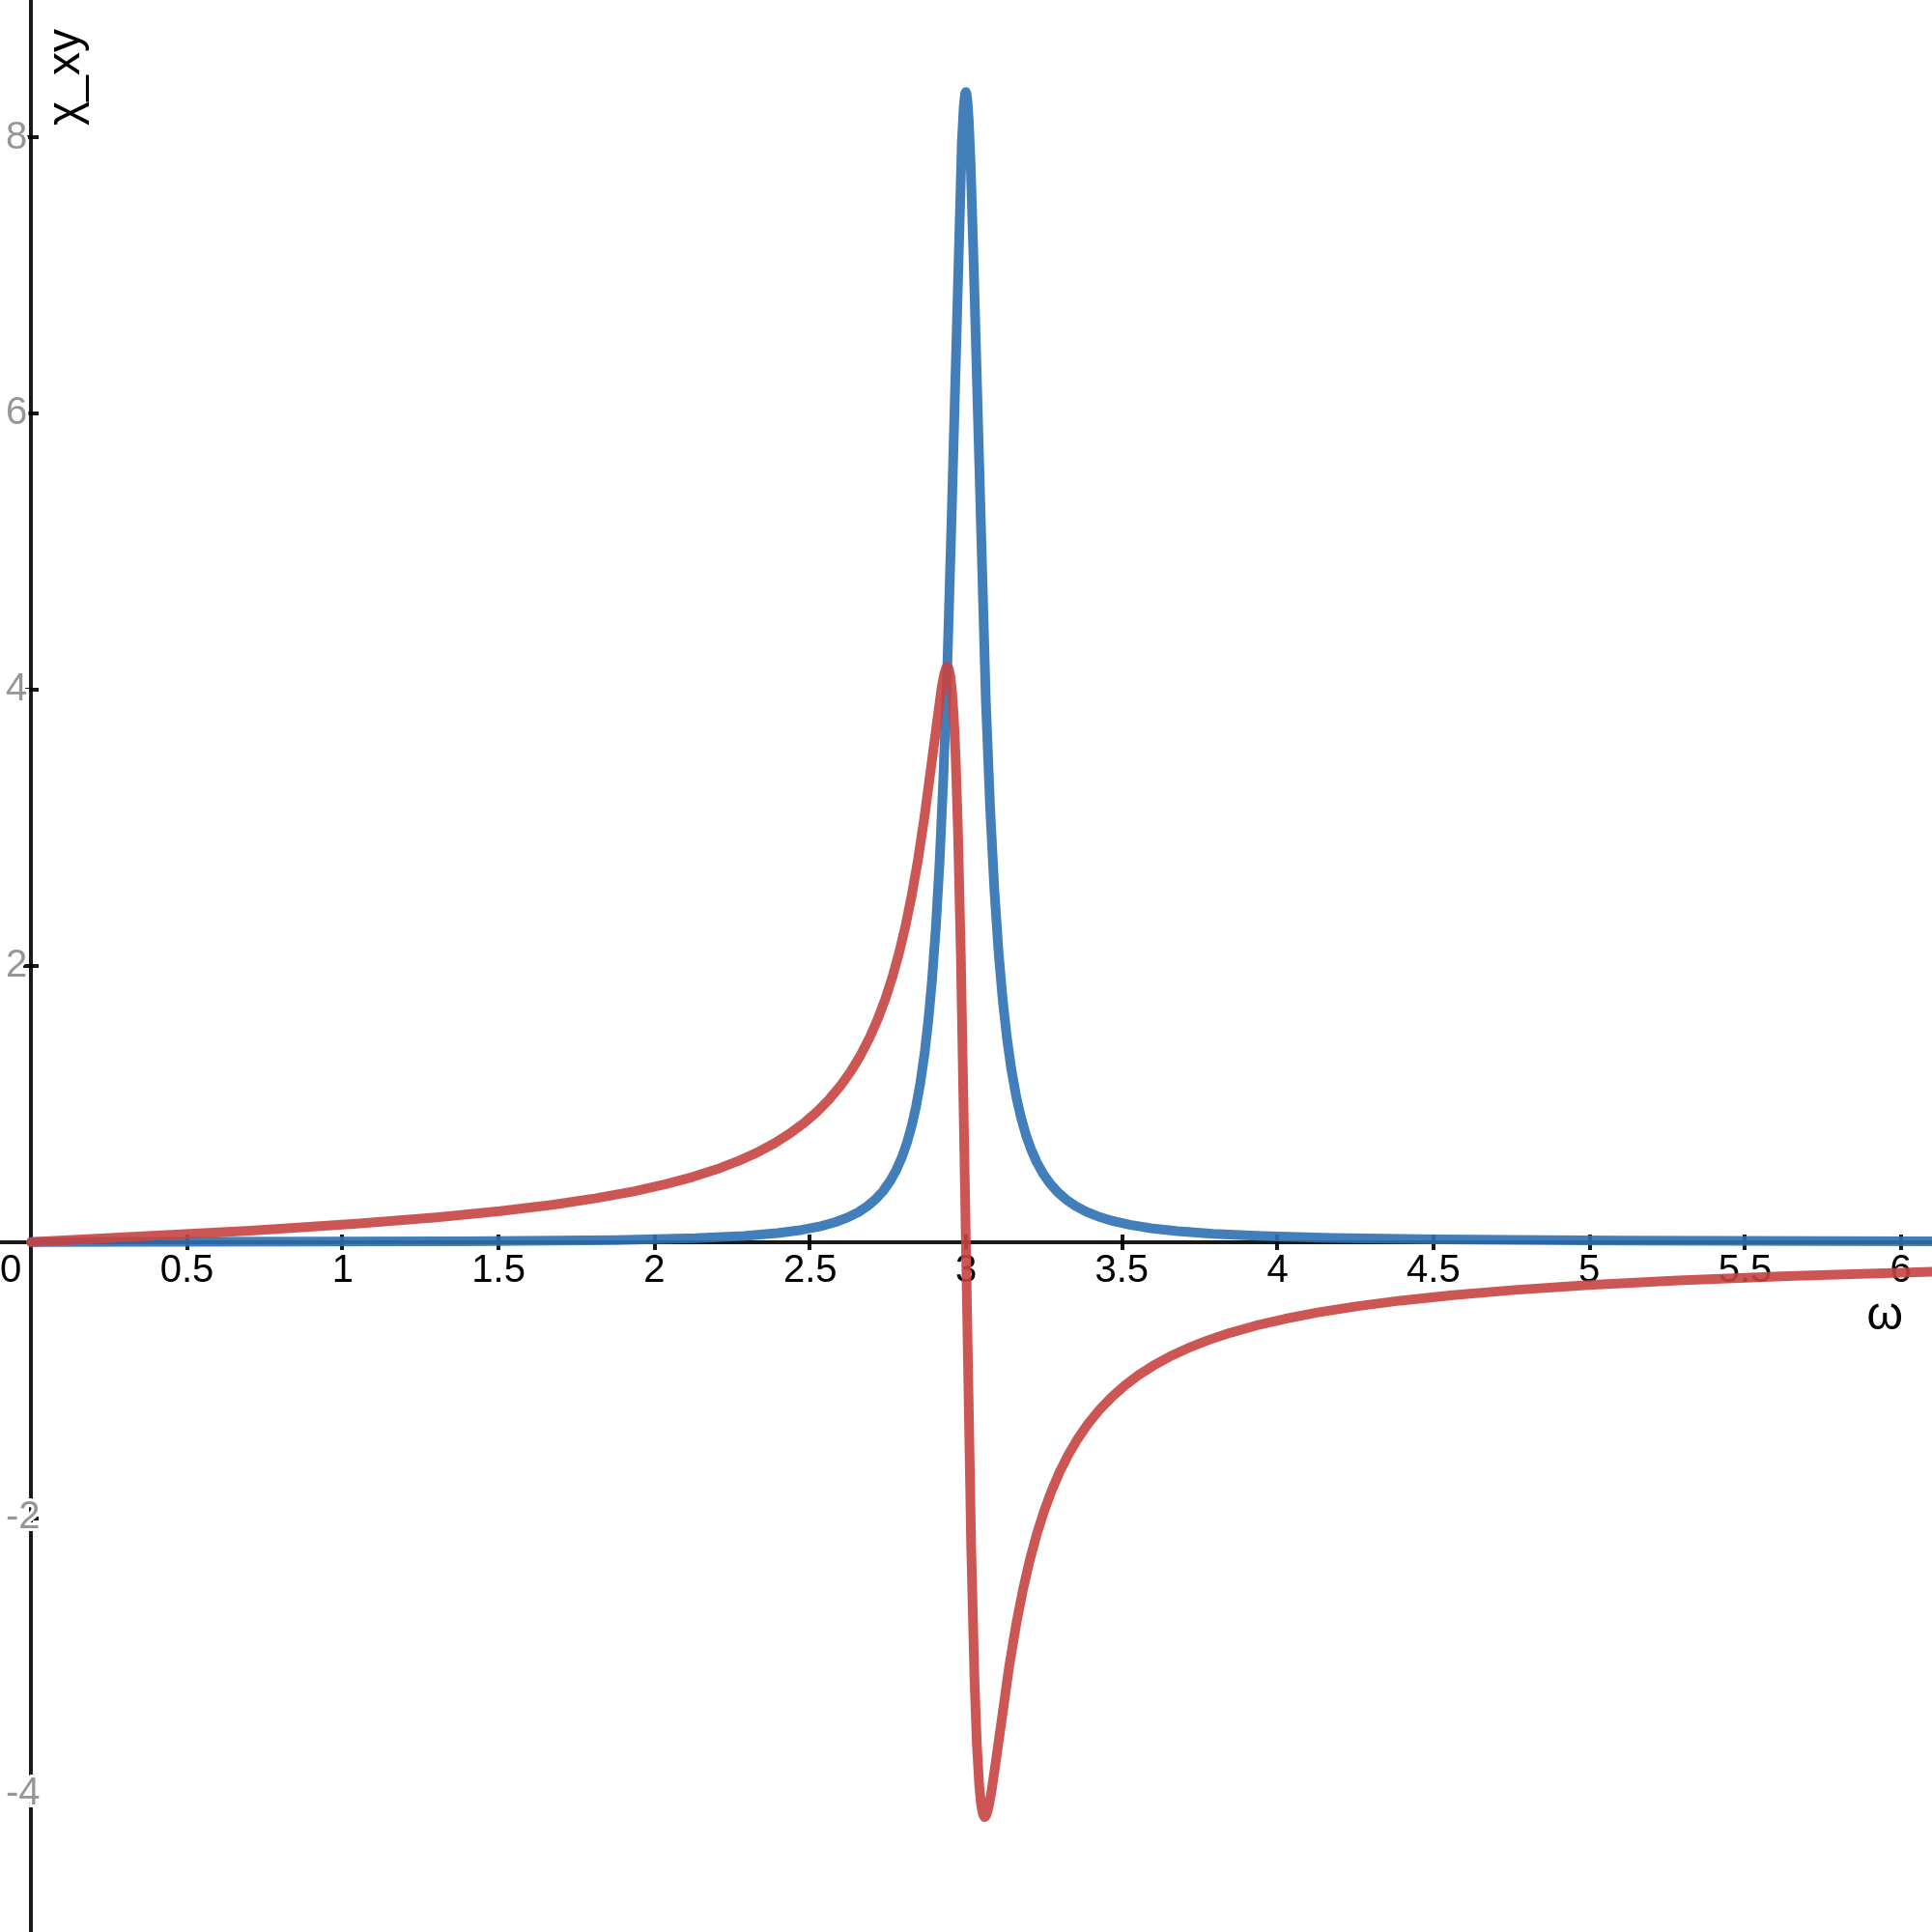
\includegraphics[width=8cm]{chi_xy.png}
  \fgcaption{$\chi_{xy}$のグラフ(青線:実部,赤線:虚部)}
\end{center}
\begin{center}
  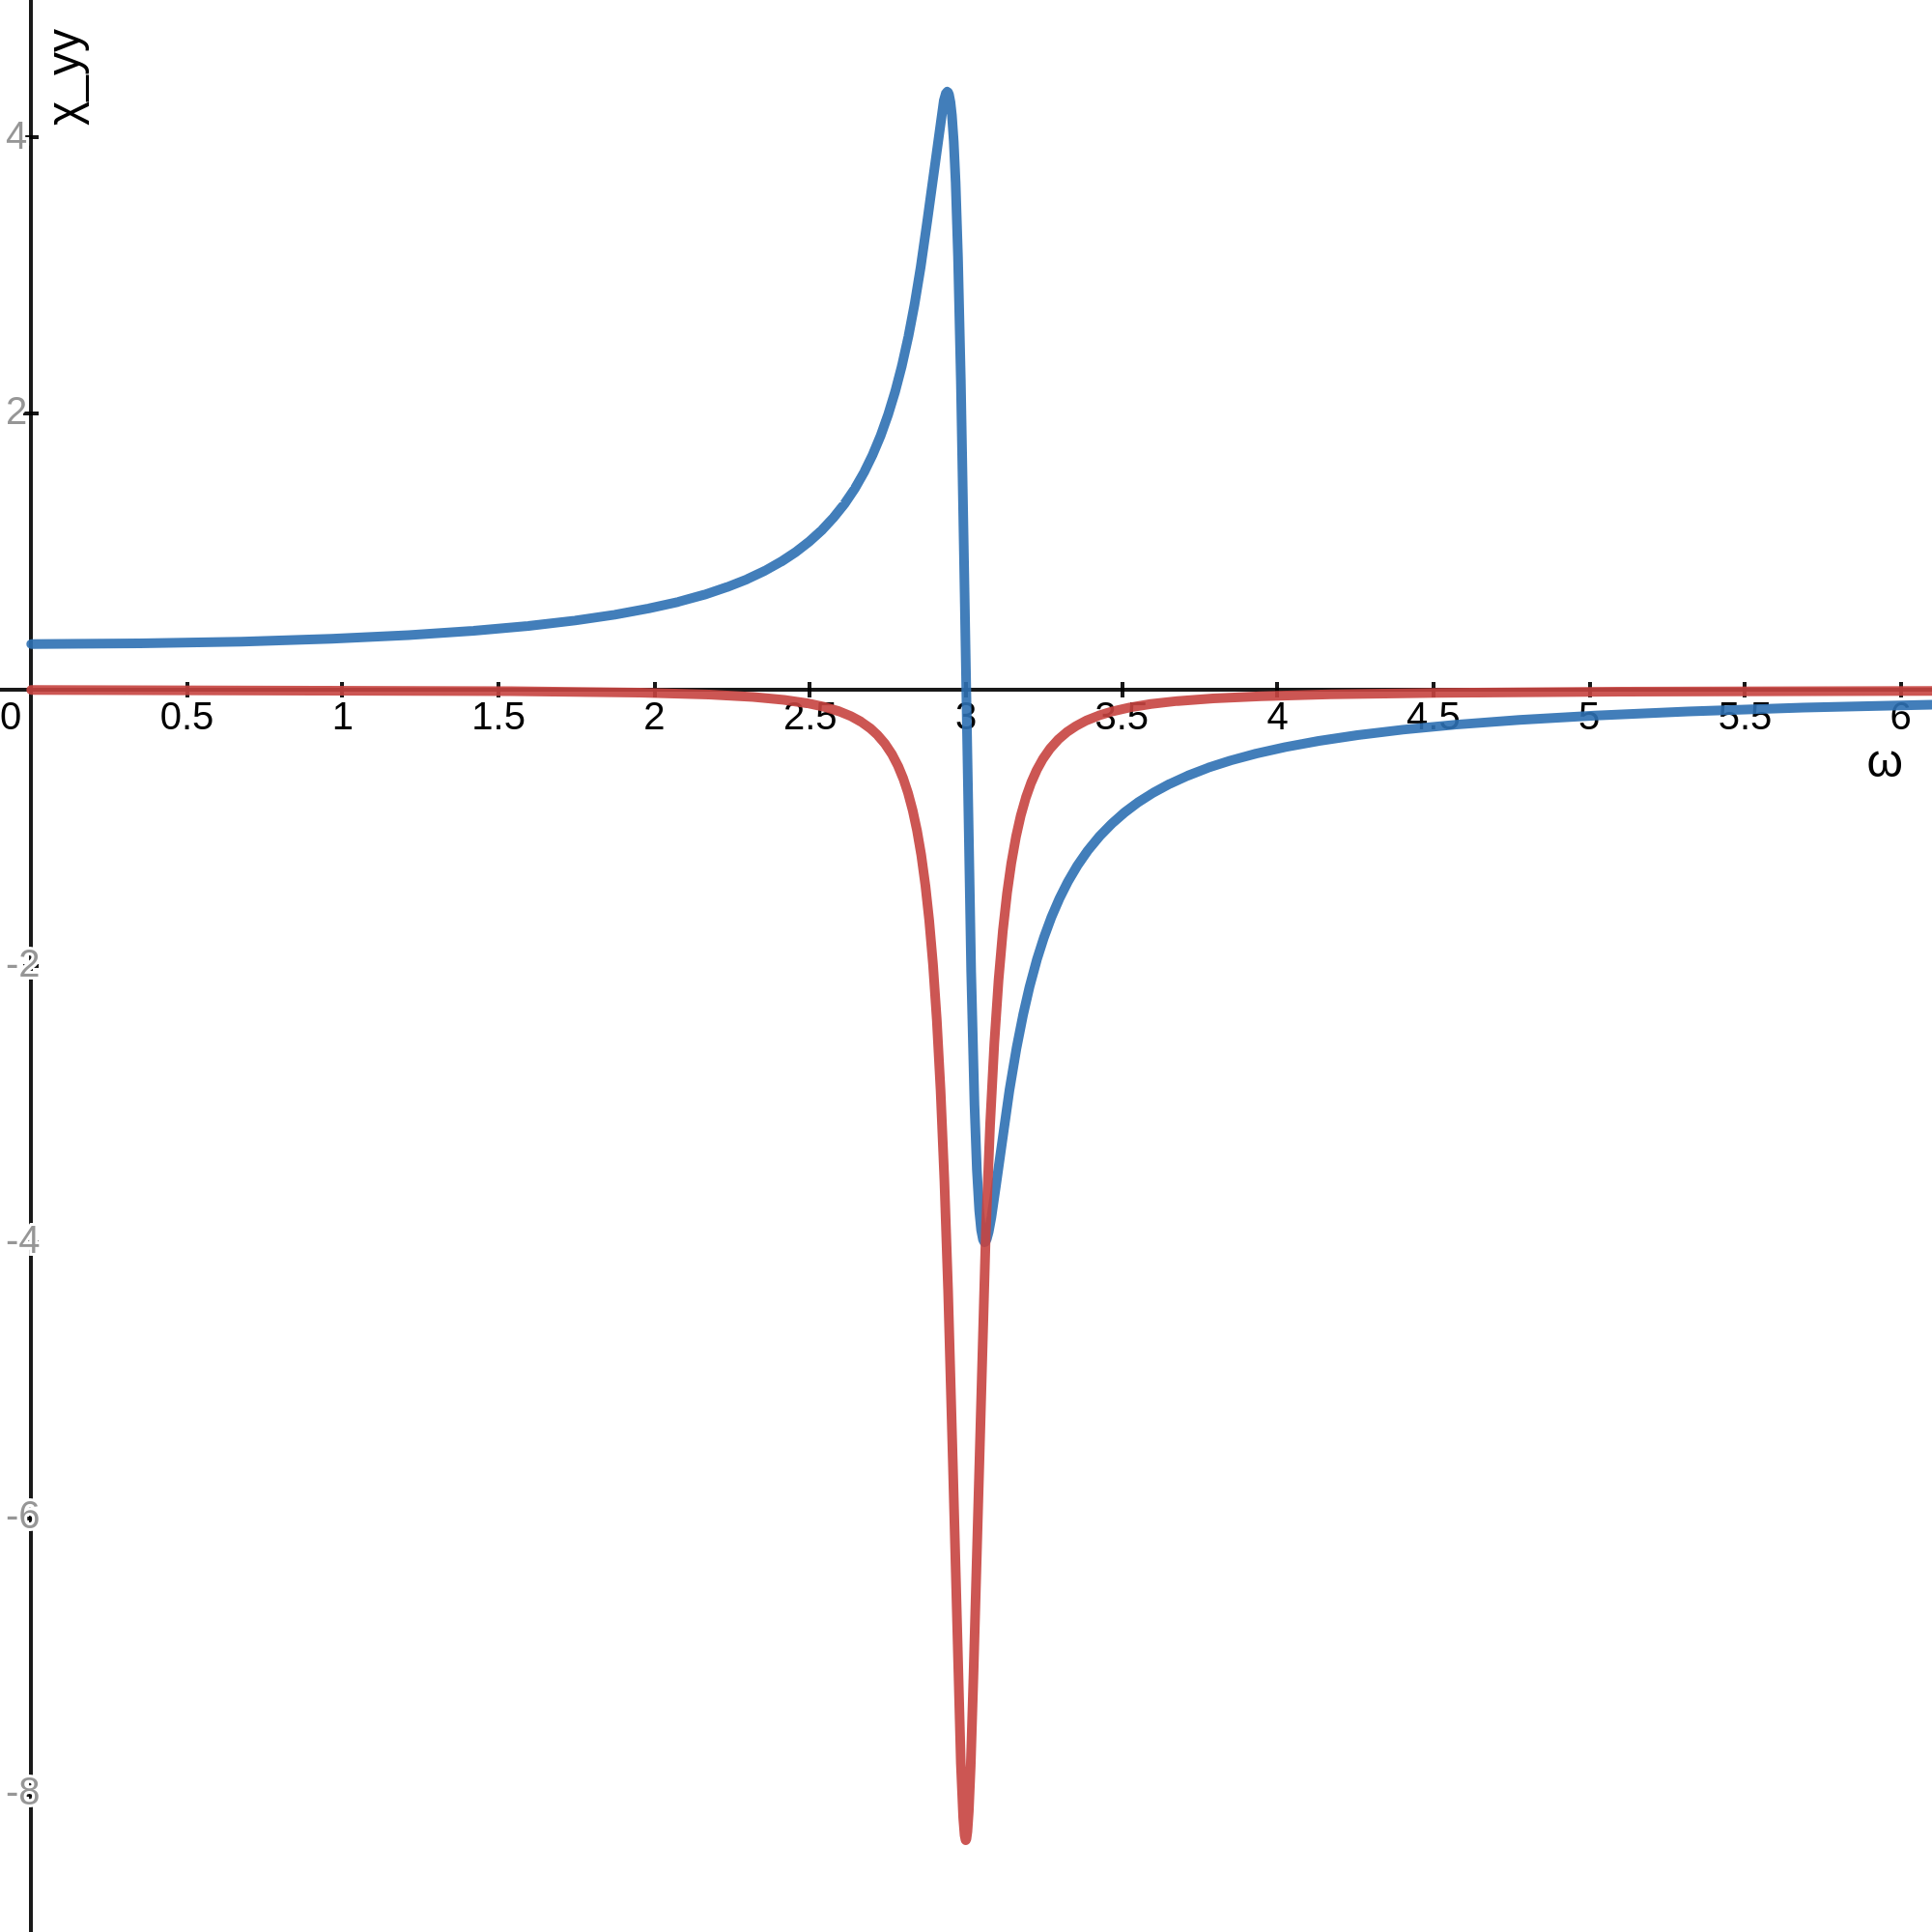
\includegraphics[width=8cm]{chi_yy.png}
  \fgcaption{$\chi_{yy}$のグラフ(青線:実部,赤線:虚部)}
\end{center}
\end{document}